\documentclass[a4paper,11pt]{article}
\usepackage[utf8]{inputenc}
\usepackage{graphicx}
\usepackage[UKenglish]{datetime}
\usepackage[top=1in, bottom=1in, right=1in, left=1in]{geometry}
\usepackage{pdfpages}
\usepackage{hyperref}

\begin{document}

\author{Minh Le Kieu \and Koen H. van Dam\and Jason Thompson \and Nick Malleson \and Alison Heppenstall \and Jiaqi Ge}
\title{International Workshop on \\ Agent-Based Modelling of Urban Systems (ABMUS) \\ Proceedings: 2022}
\date{Tuesday 10th May 2022}

\maketitle
\newpage
\tableofcontents

\newpage

\section{Session 1: Methodology}

\subsection{Synthetic generation of individual transport data: the case of Smart Card data
 \\ Minh Kieu, Iris Meredith and Andrea Raith}
 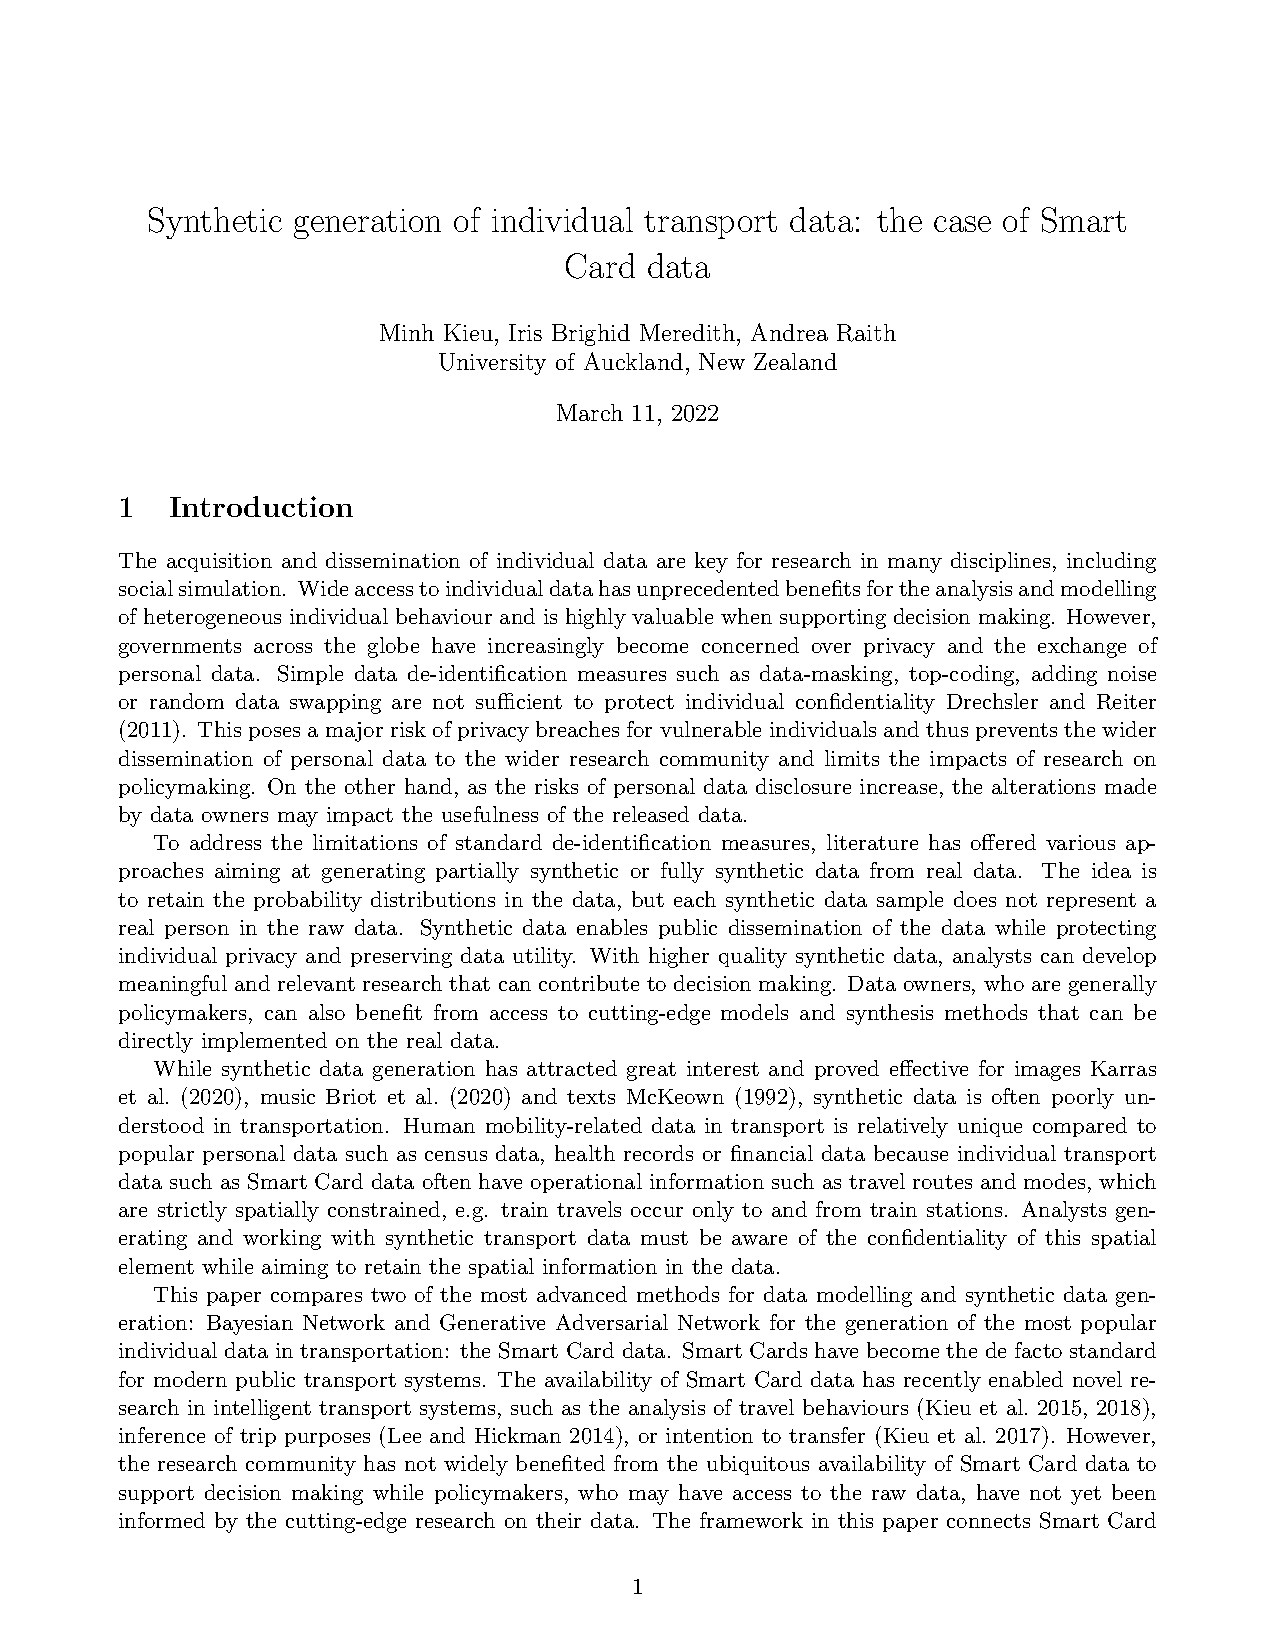
\includepdf[pages=-]{ABMUS2022_paper_8.pdf}

\subsection{Data-driven agent-based model development to support human-centric TOD design \\ Liu Yang and Koen van Dam. }
 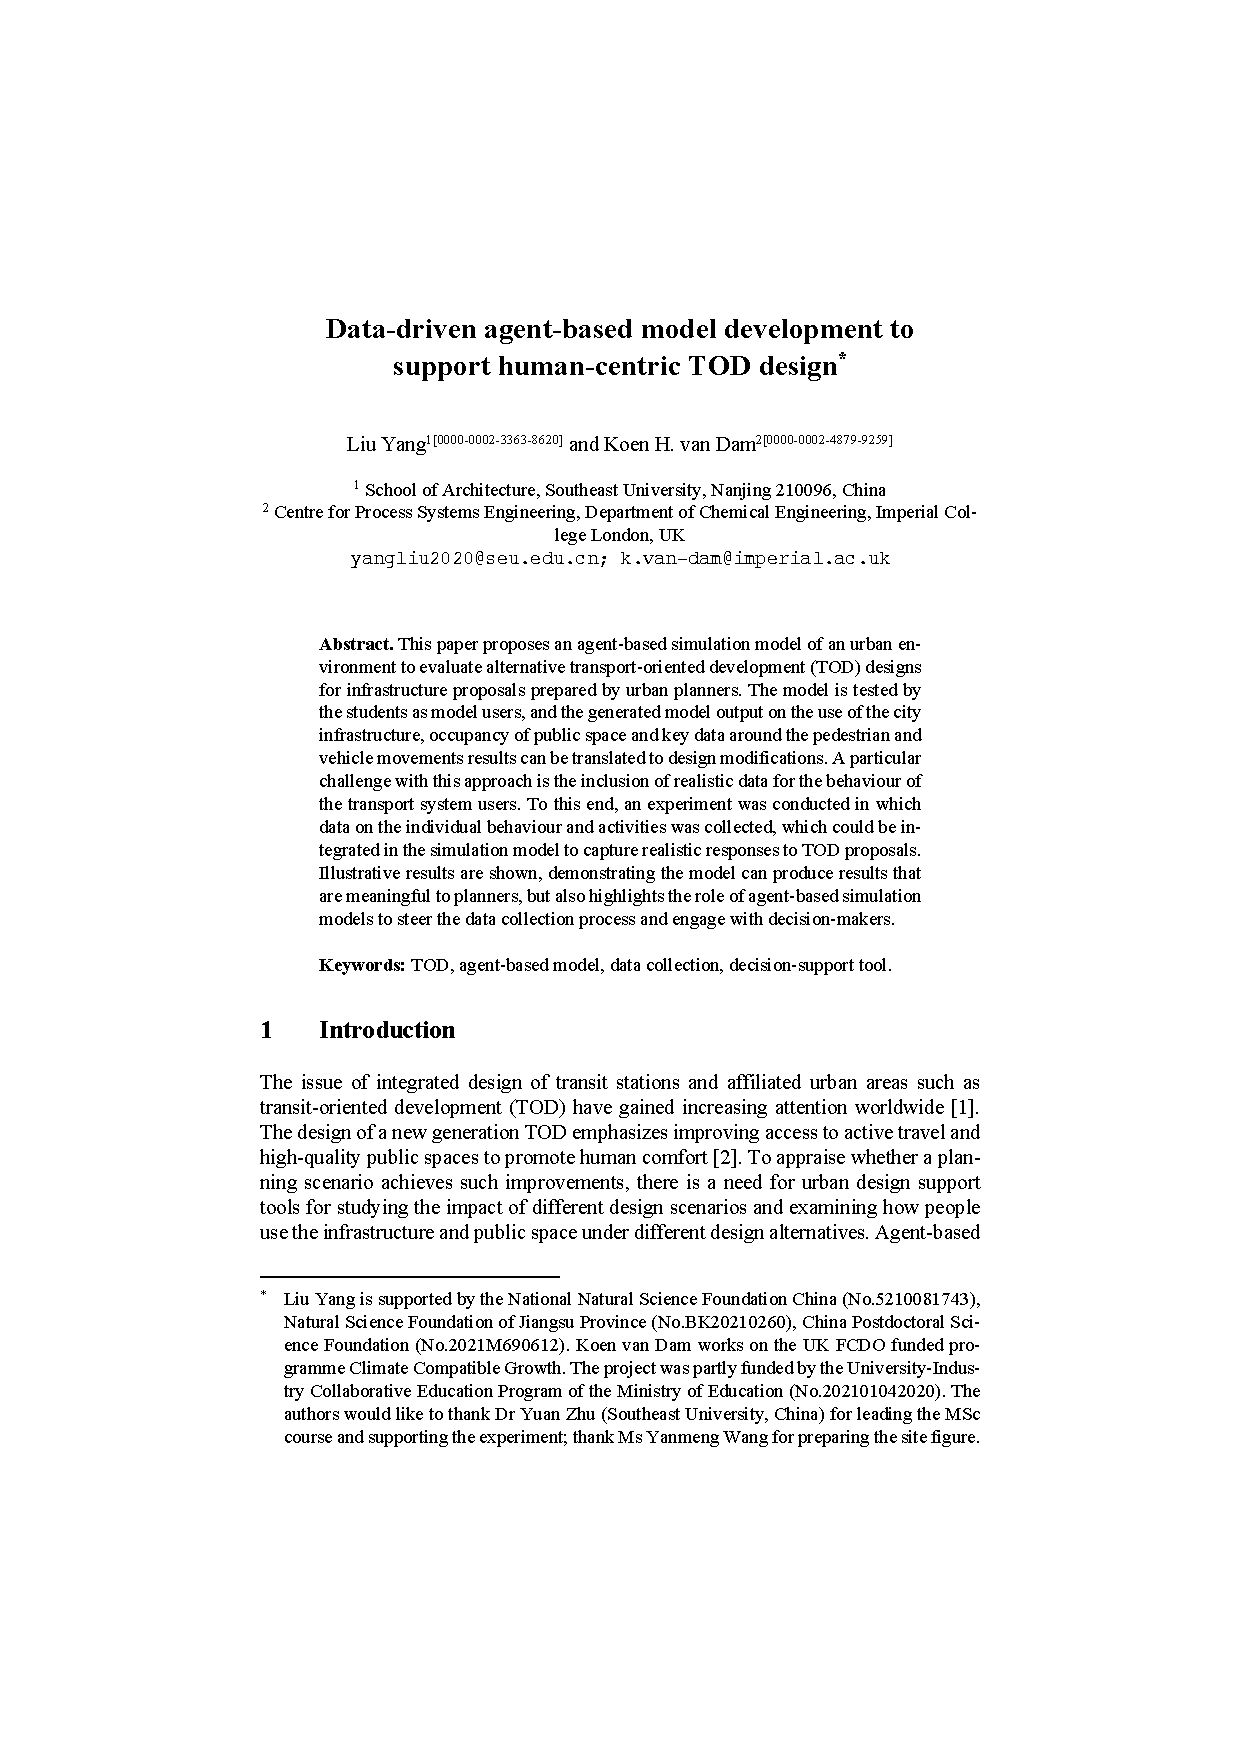
\includepdf[pages=-]{ABMUS2022_paper_5.pdf}

\subsection{AgentsX.jl — An Extended Julia Framework for Exploring Urban and Social Systems \\ Rajith Vidanaarachchi, Jason Thompson, Branislava Godic and Rod McClure}
 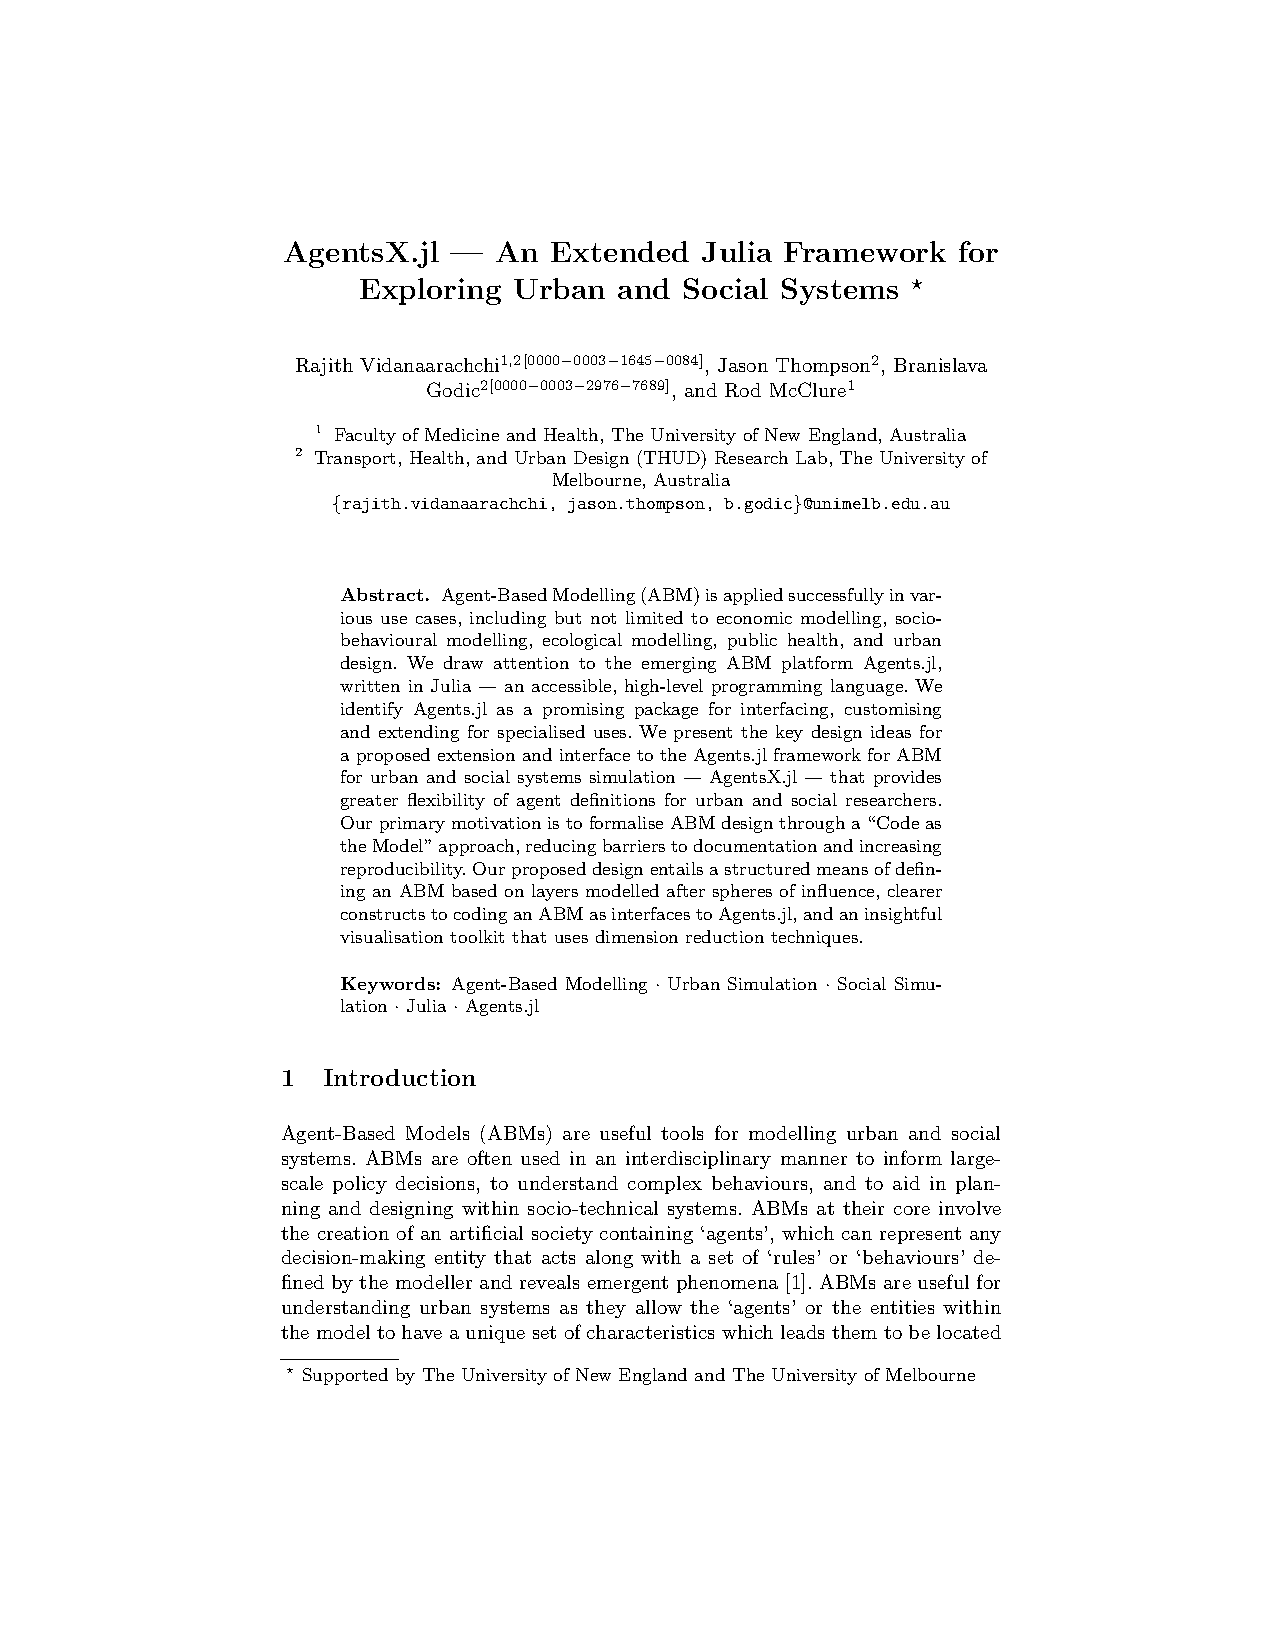
\includepdf[pages=-]{ABMUS2022_paper_9.pdf}

\subsection{Simulating civil emergency evacuation with Inverse Generative Social Science \\ Gayani Senanayake and Minh Kieu}
 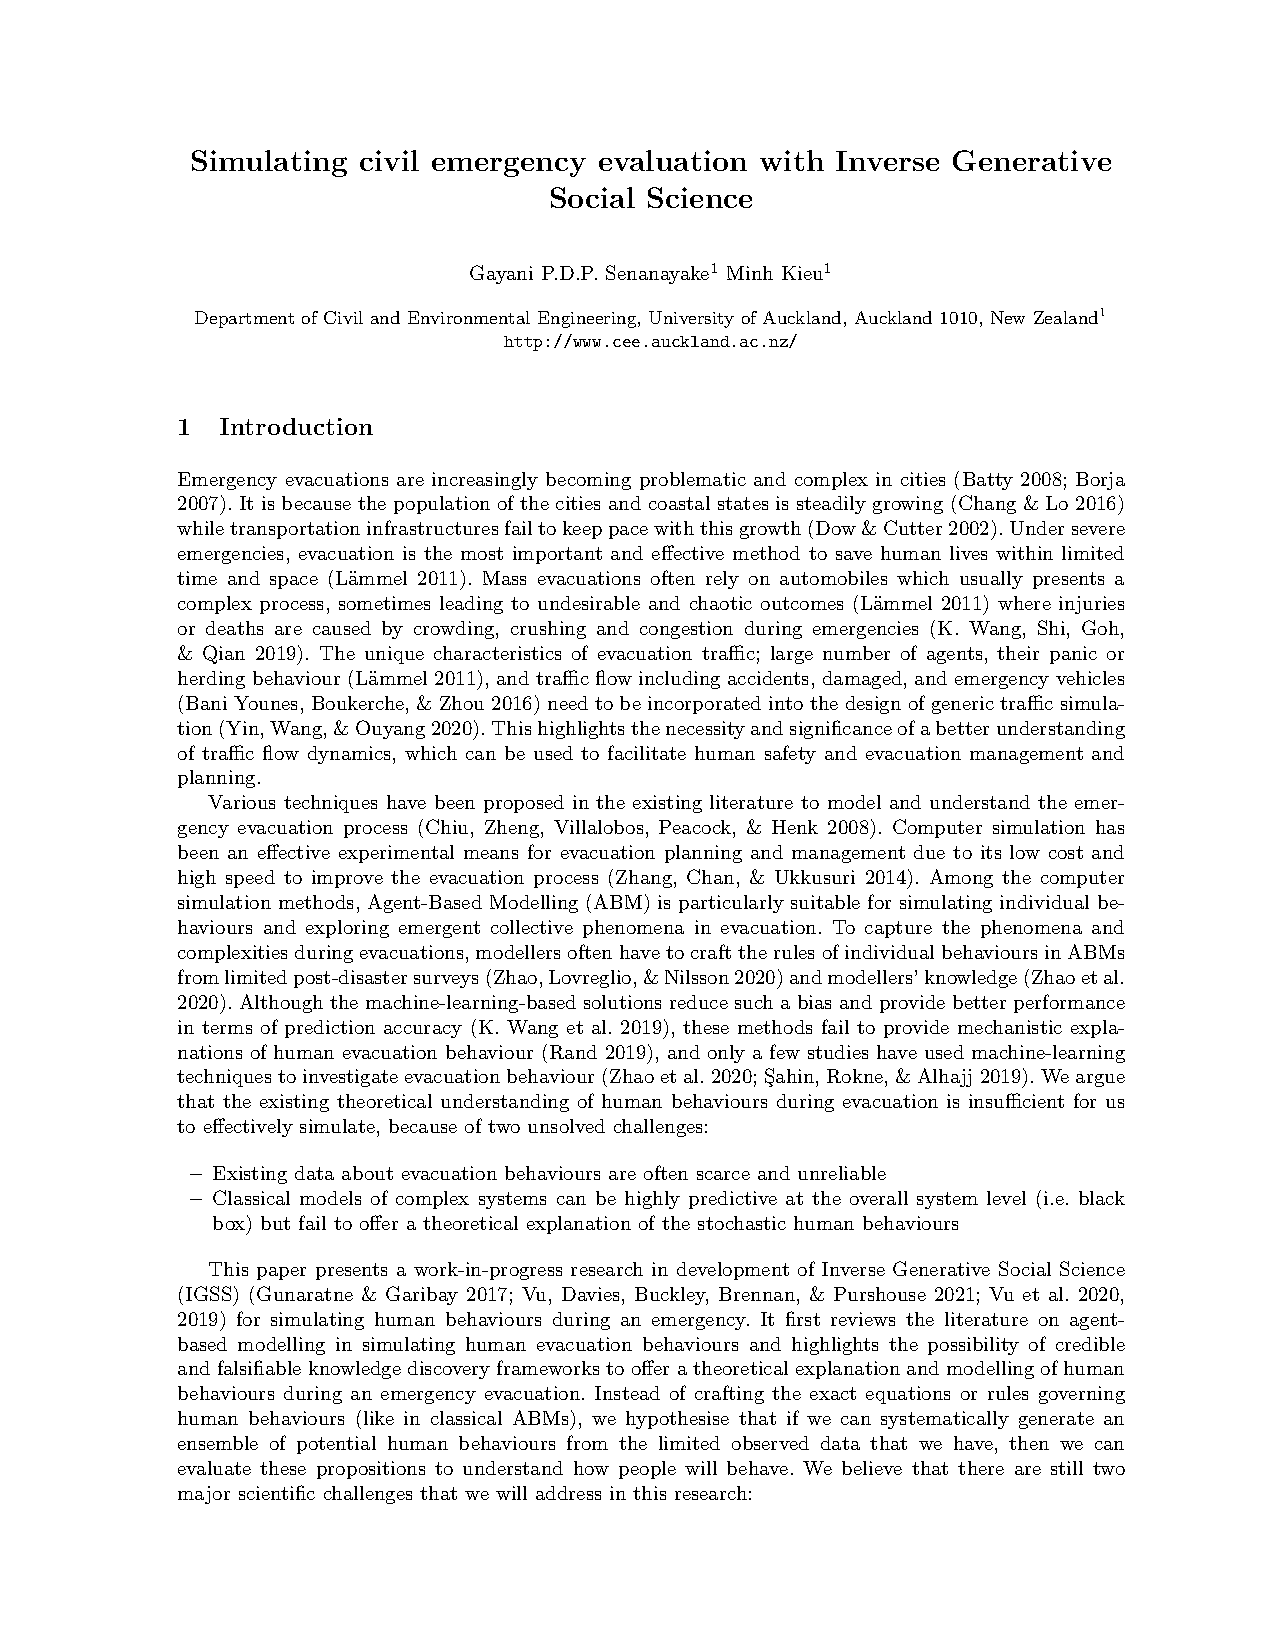
\includepdf[pages=-]{ABMUS2022_paper_12.pdf}


\section{Session 2: Urban Development}

\subsection{No Hope for First-Time Buyers? Towards Agent-Based Market Analysis of Urban Housing Balance \\ Erik Wiegel and Neil Yorke-Smith. }
 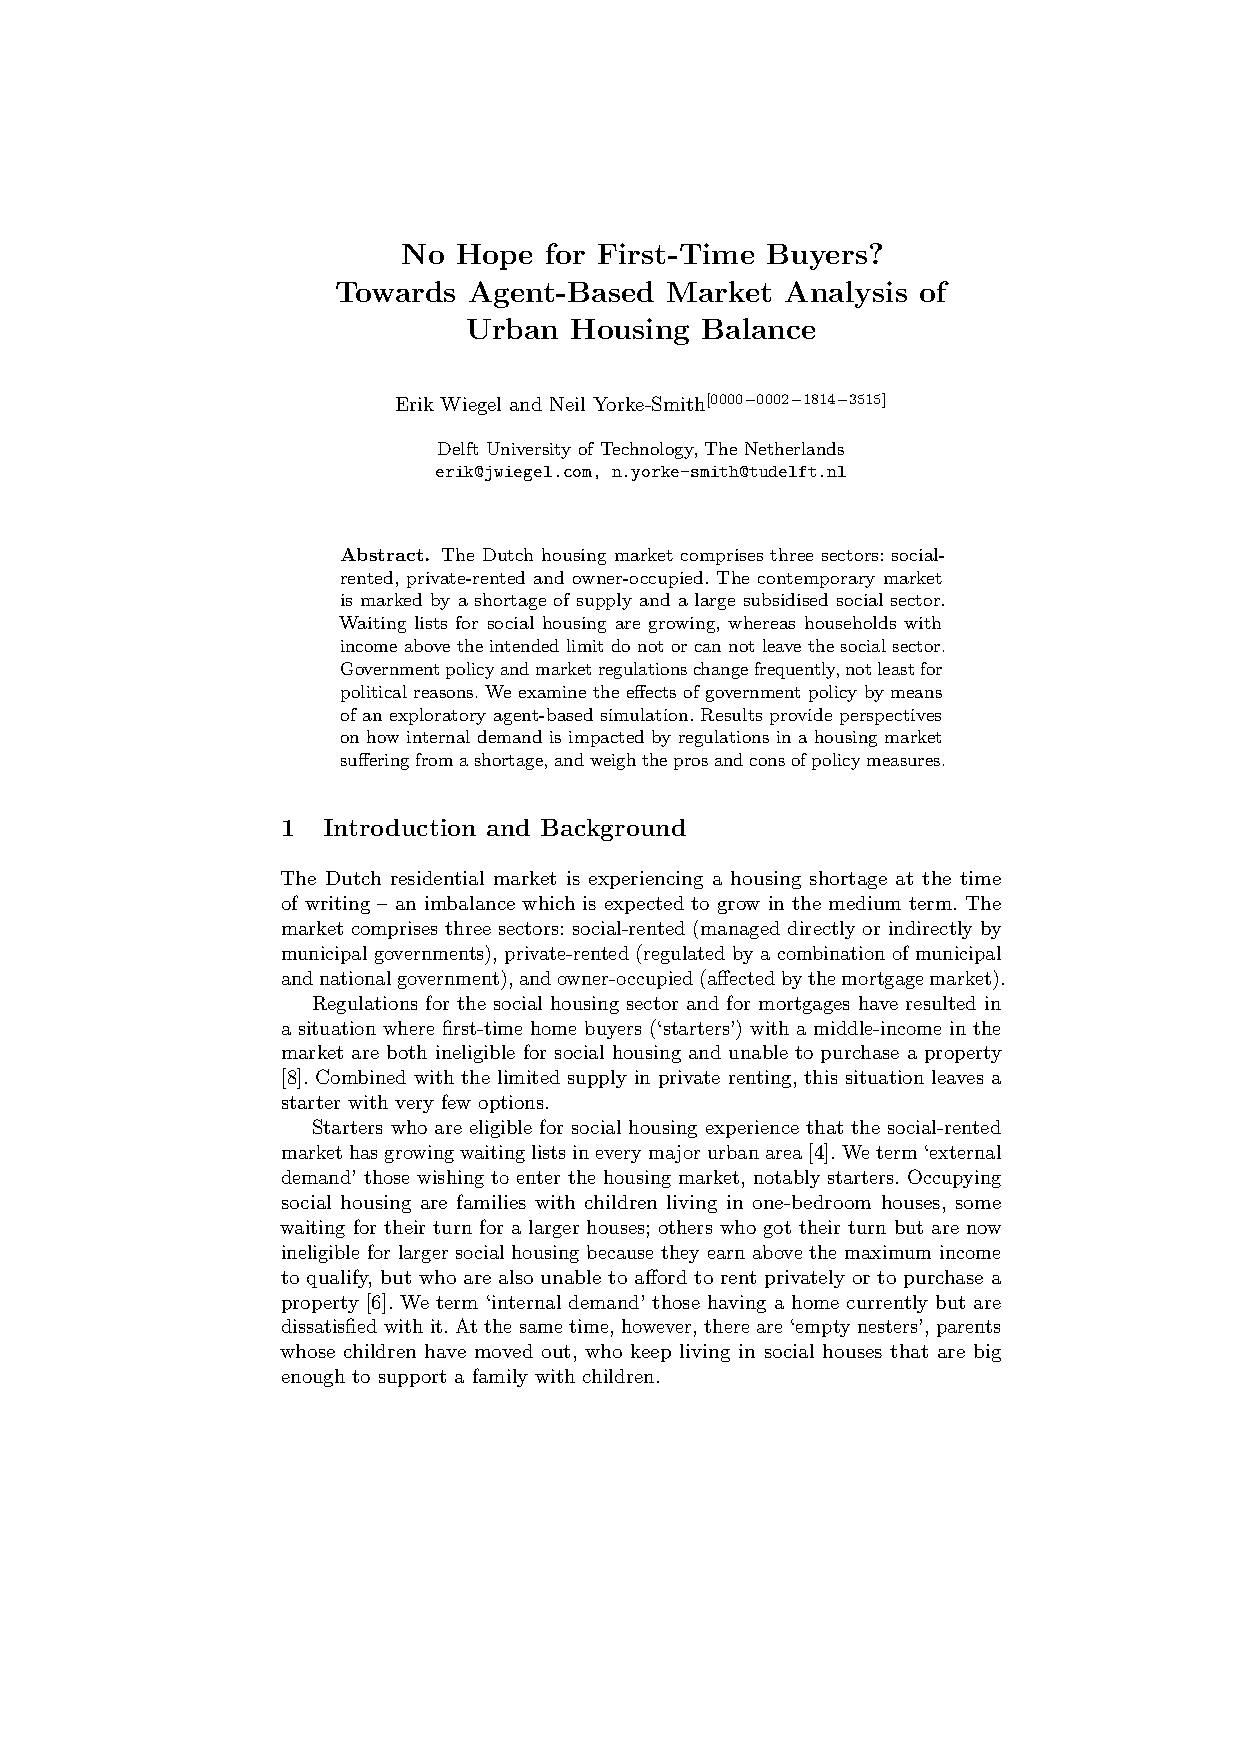
\includepdf[pages=-]{ABMUS2022_paper_1.pdf}
 
 \subsection{Agent-Based Modelling of People's Behaviour in Public Parks \\ Sabine Timpf and Marie-Rose Degg. }
 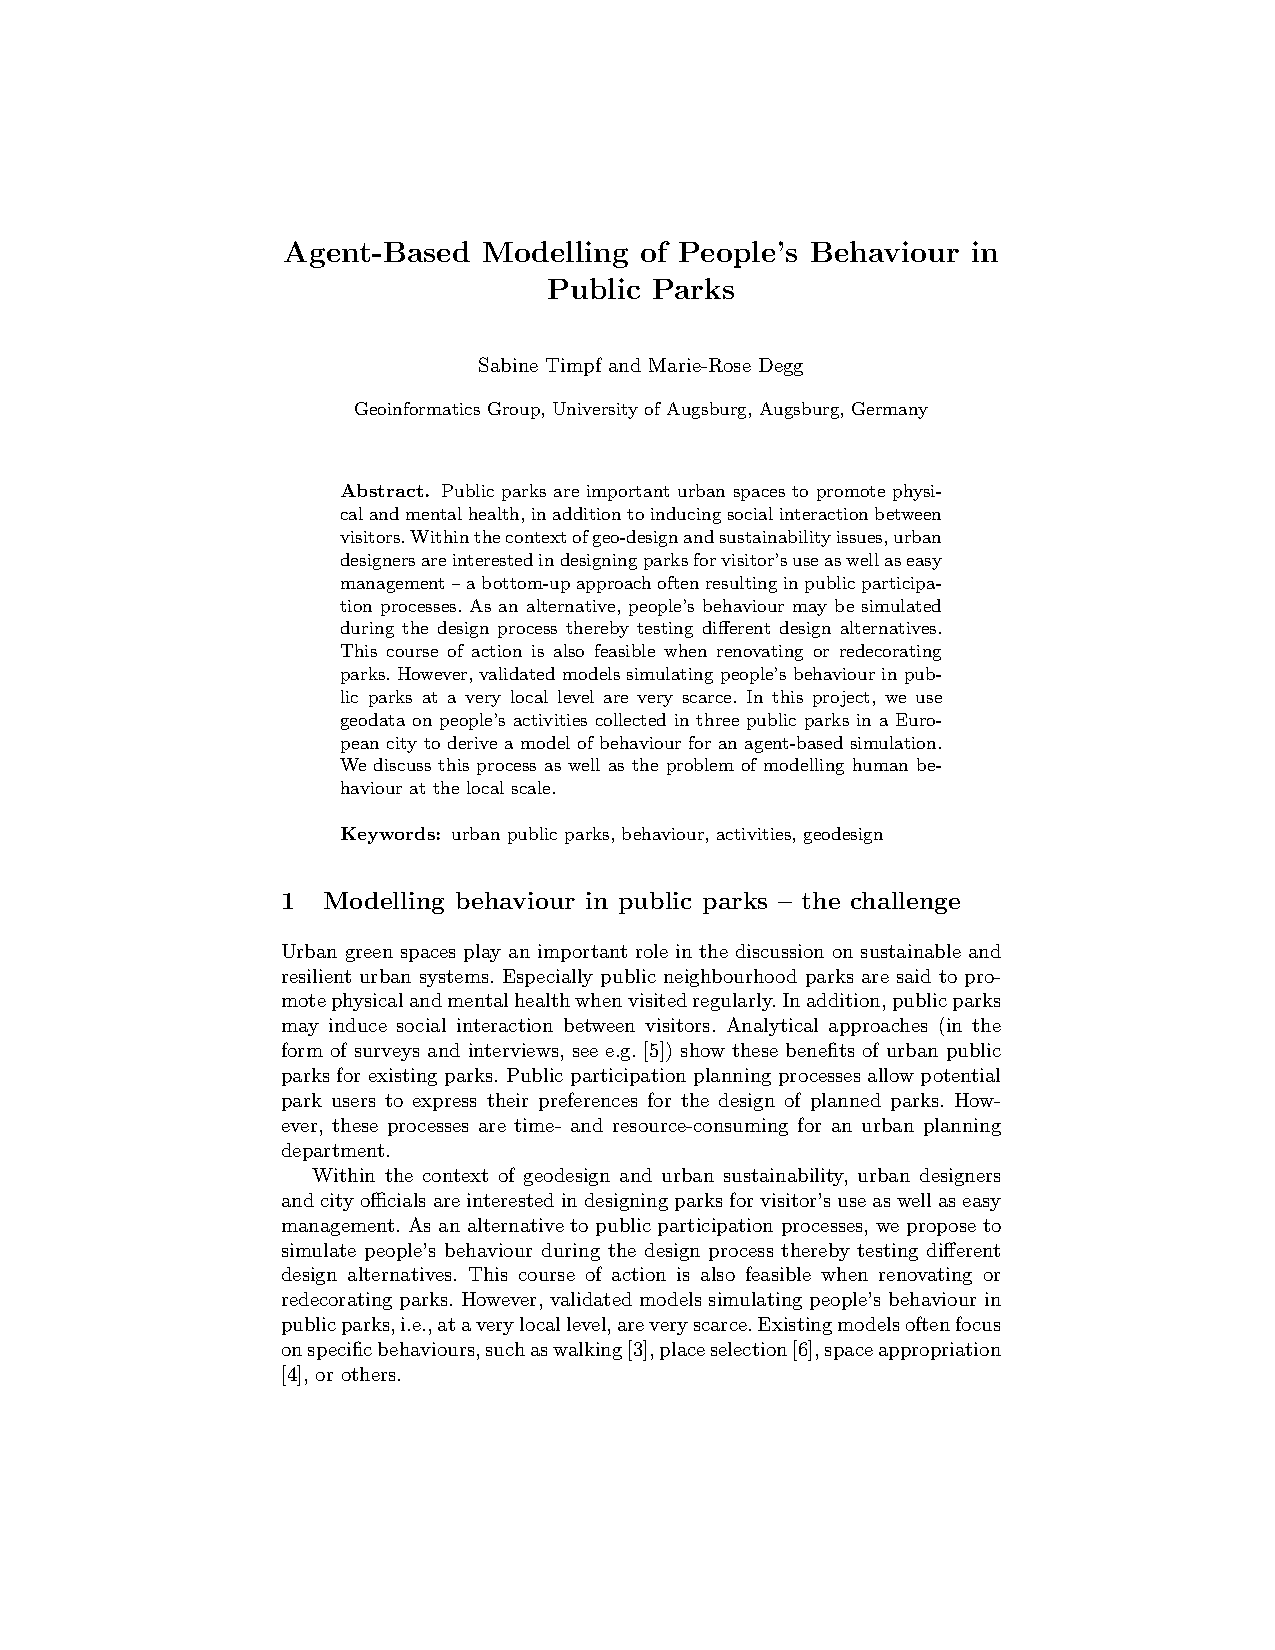
\includepdf[pages=-]{ABMUS2022_paper_11.pdf}
 
 \subsection{An agent-based model of greening a city for reducing pluvial flooding at a cultural heritage site \\ Emily West, Rembrandt Koppelaar, Aitziber Egusquiza Ortega, Angela Santangelo and Eleonora Melandri.}
 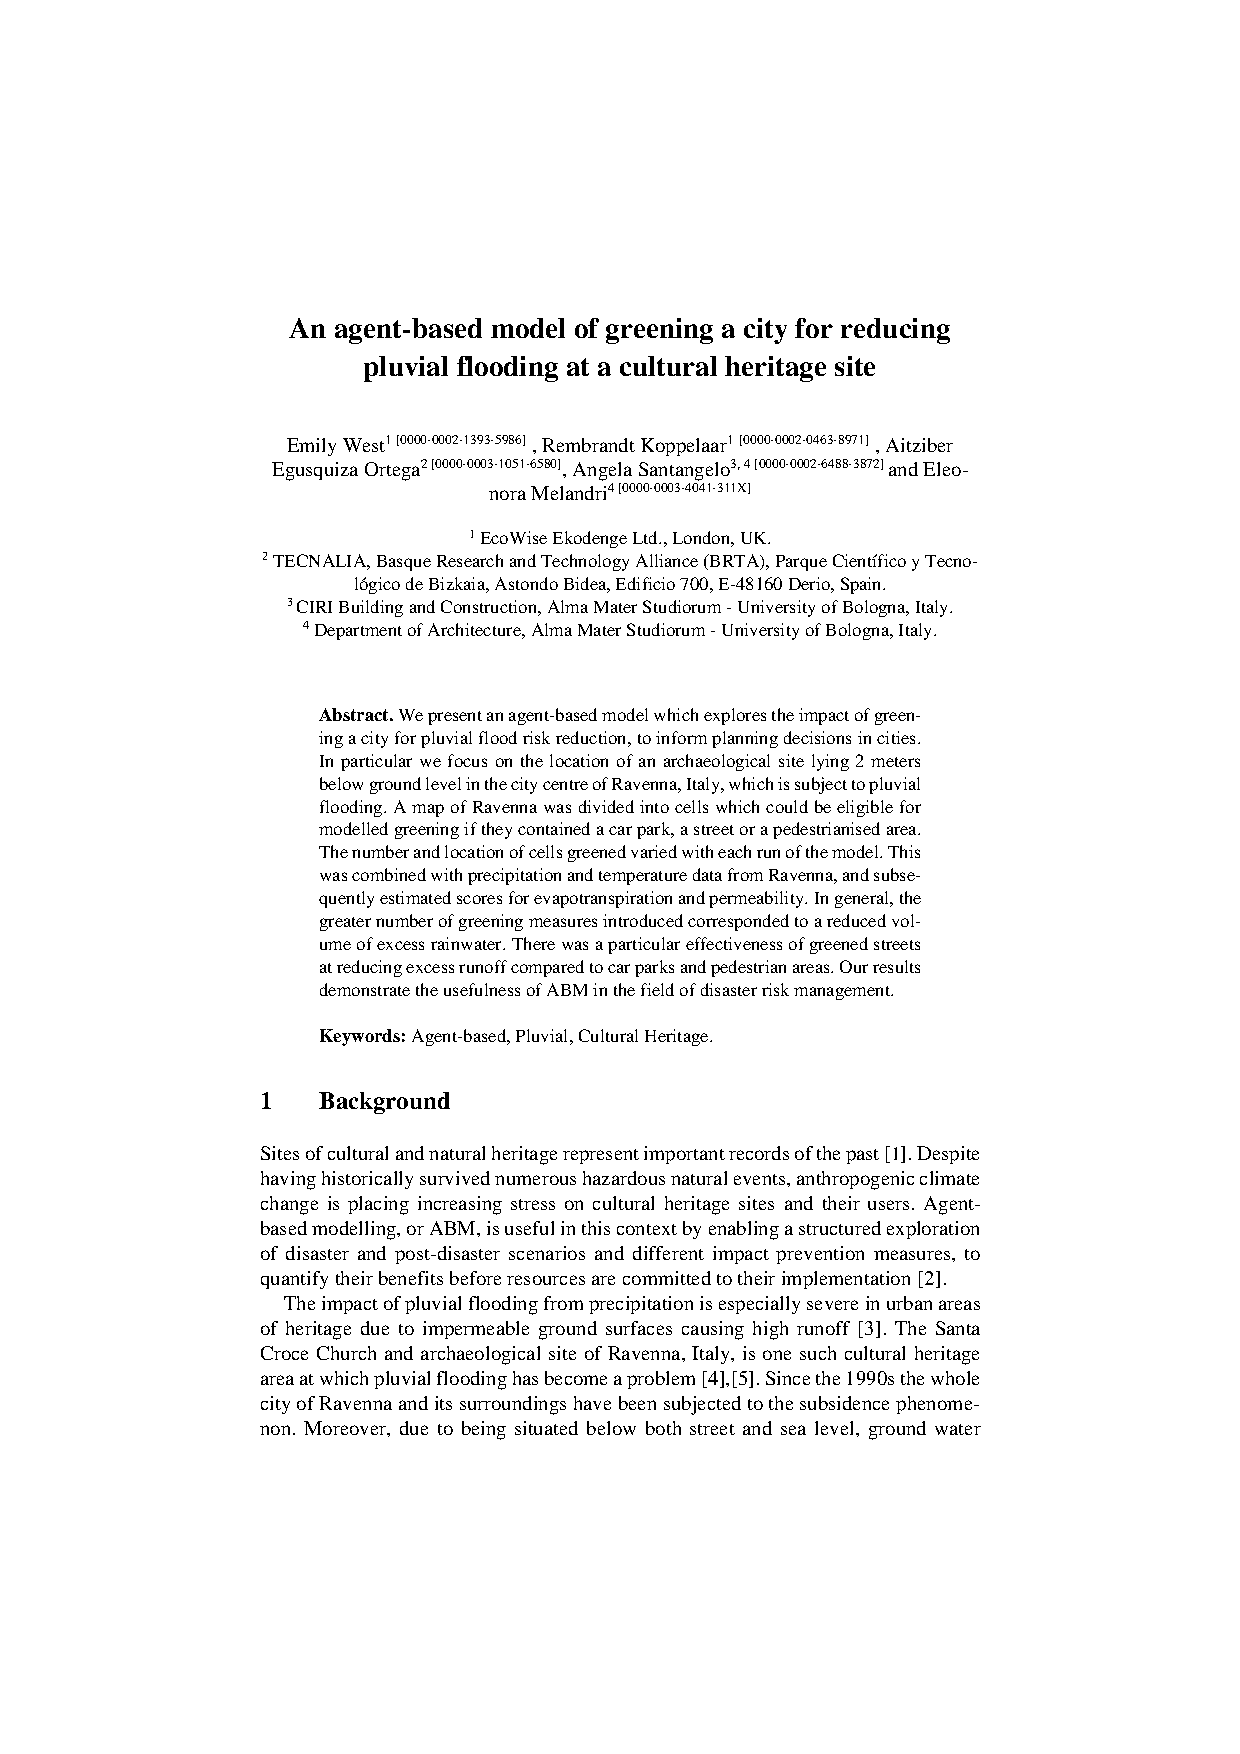
\includepdf[pages=-]{ABMUS2022_paper_2.pdf}
 
 \subsection{Real World Traffic Optimization by Reinforcement Learning: A Concept \\ Henri Meeß, Jeremias Gerner, Daniel Hein, Stefanie Schmidtner and Gordon Elger. }
 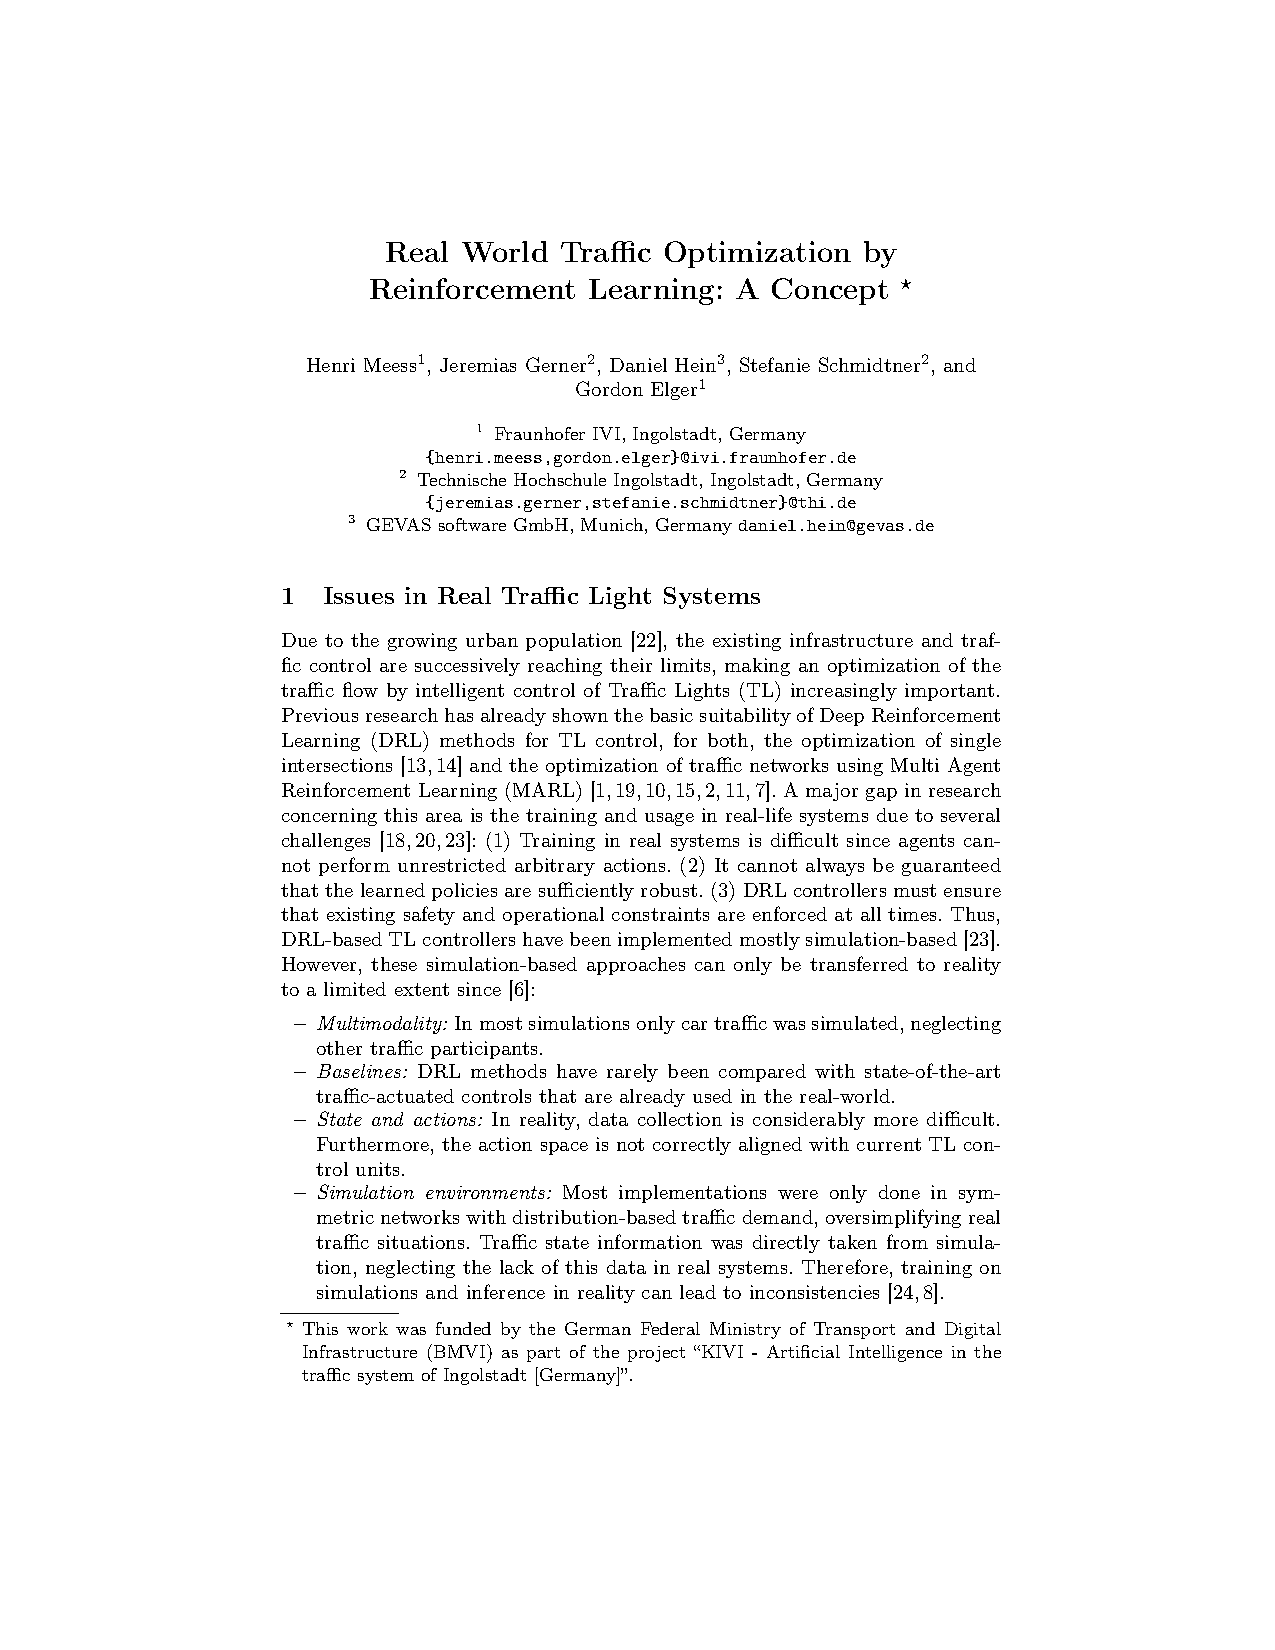
\includepdf[pages=-]{ABMUS2022_paper_4.pdf}

\section{Session 3: Transport}

\subsection{Transport electrification and fast-charging expansion: A case study in Alaska \\ Ilya Turchaninov, Koen van Dam, Gonzalo Bustos Turu and Salvador Acha.}
 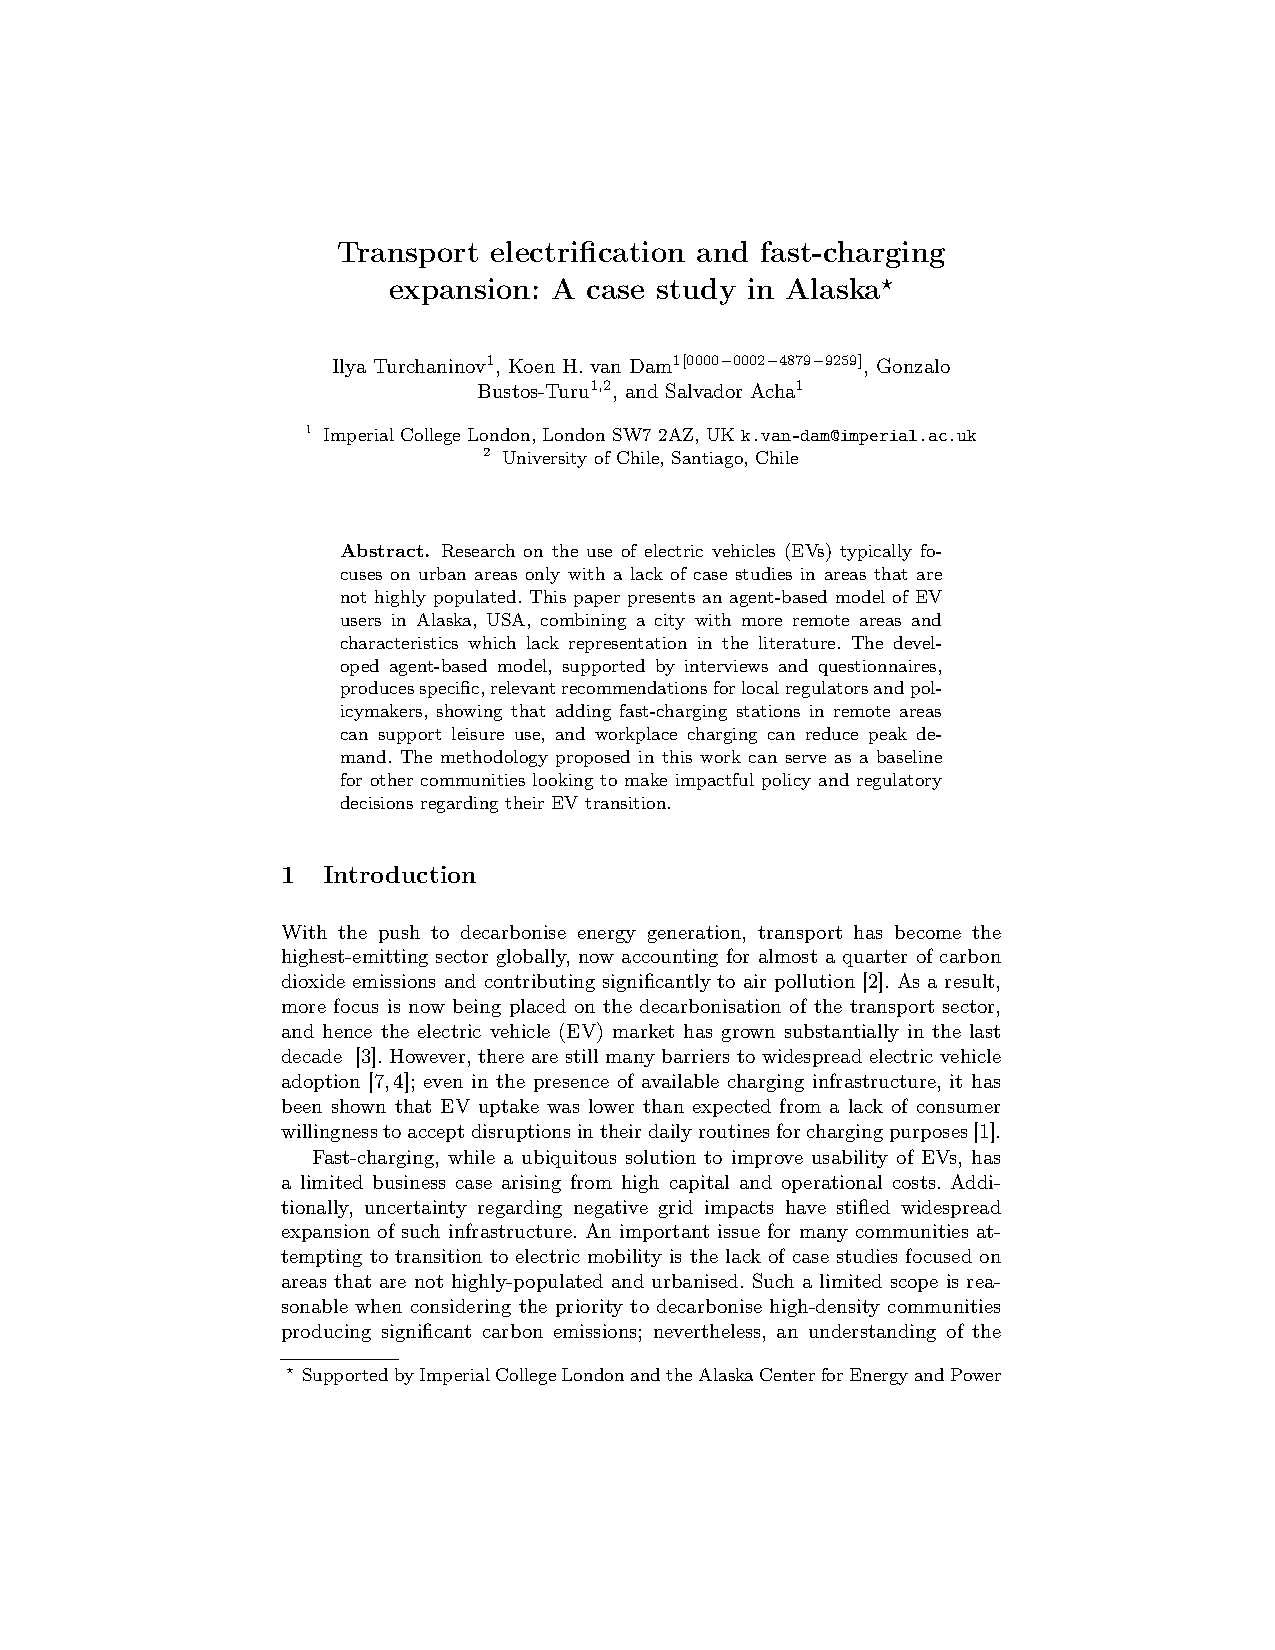
\includepdf[pages=-]{ABMUS2022_paper_10.pdf}
 
 \subsection{Learning a Robust Multiagent Driving Policy for Traffic Congestion Reduction \\ Yulin Zhang, William Macke, Jiaxun Cui, Daniel Urieli and Peter Stone}
 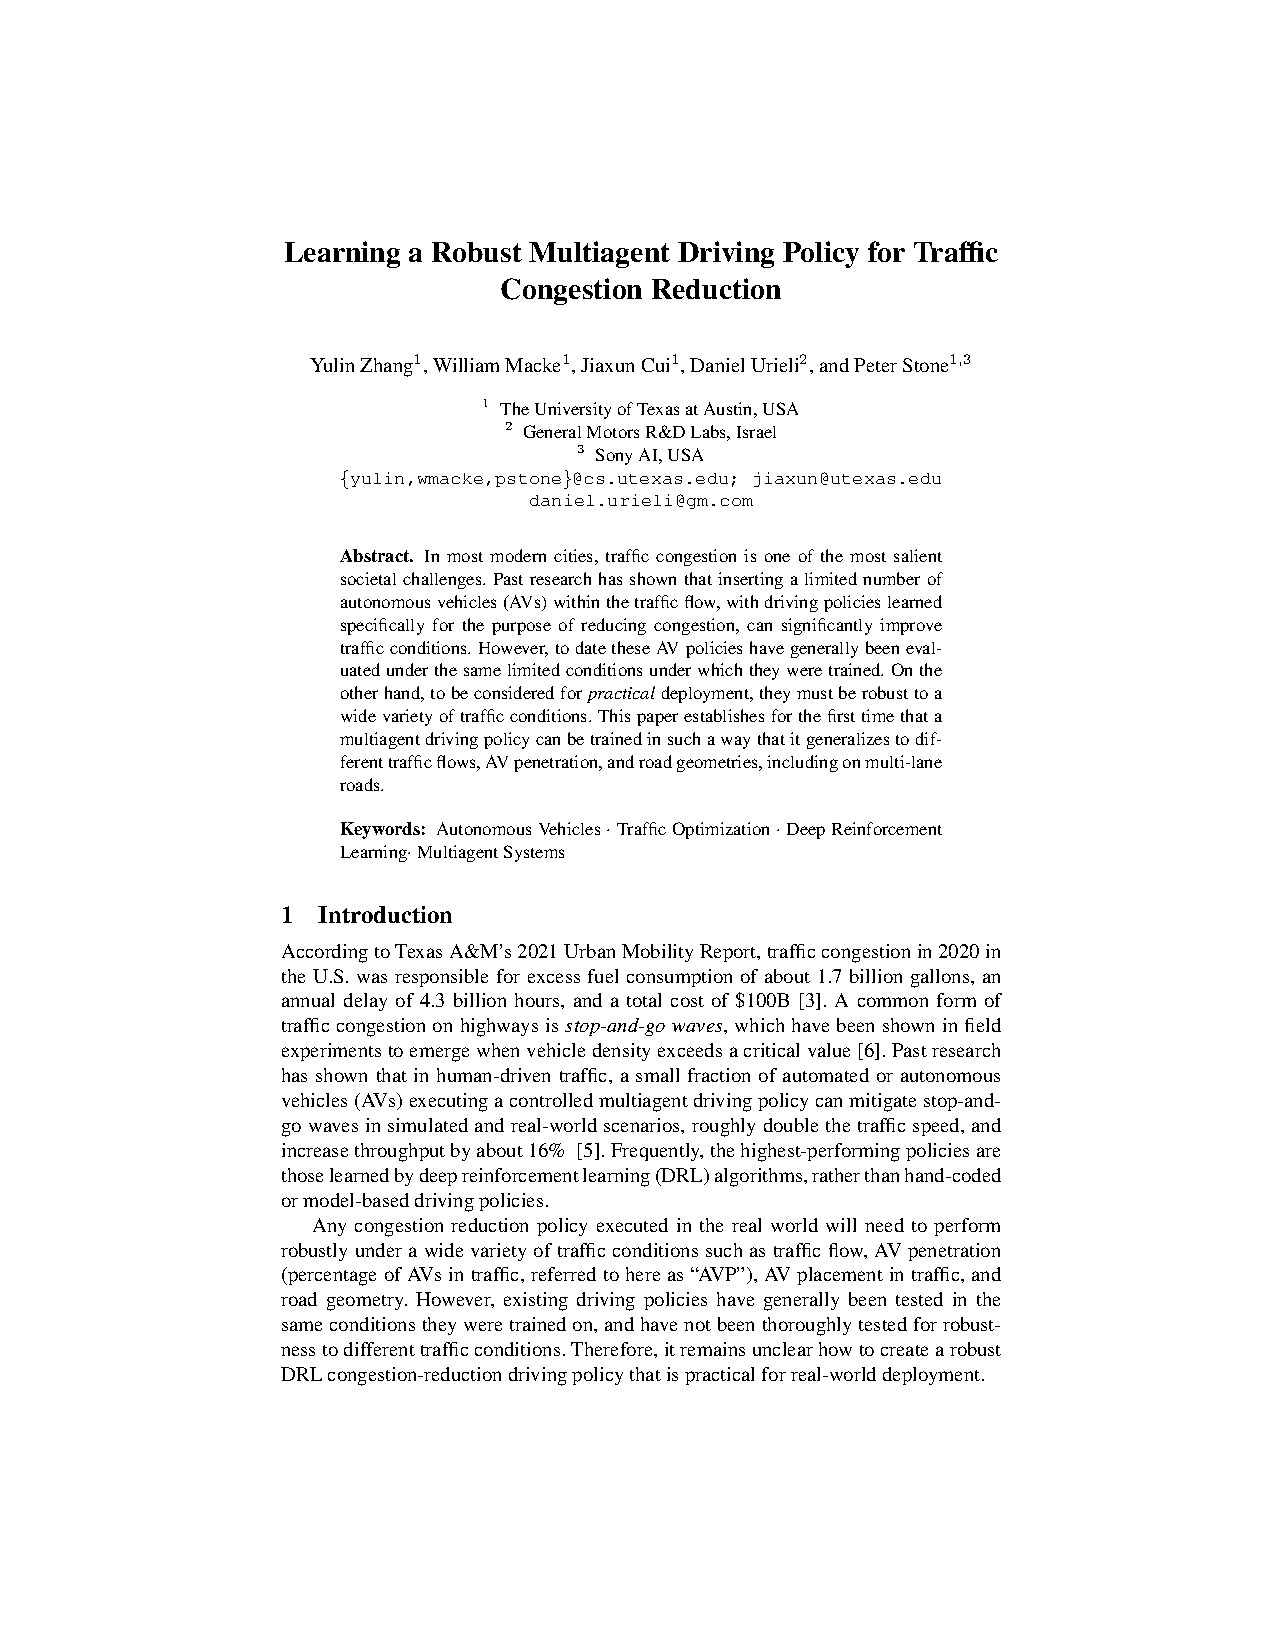
\includepdf[pages=-]{ABMUS2022_paper_3.pdf}
 
 \subsection{Preference-Aware Dynamic Ridesharing \\ Yi Cheng Ong, Nicos Protopapas, Vahid Yazdanpanah, Enrico H. Gerding and Sebastian Stein}
 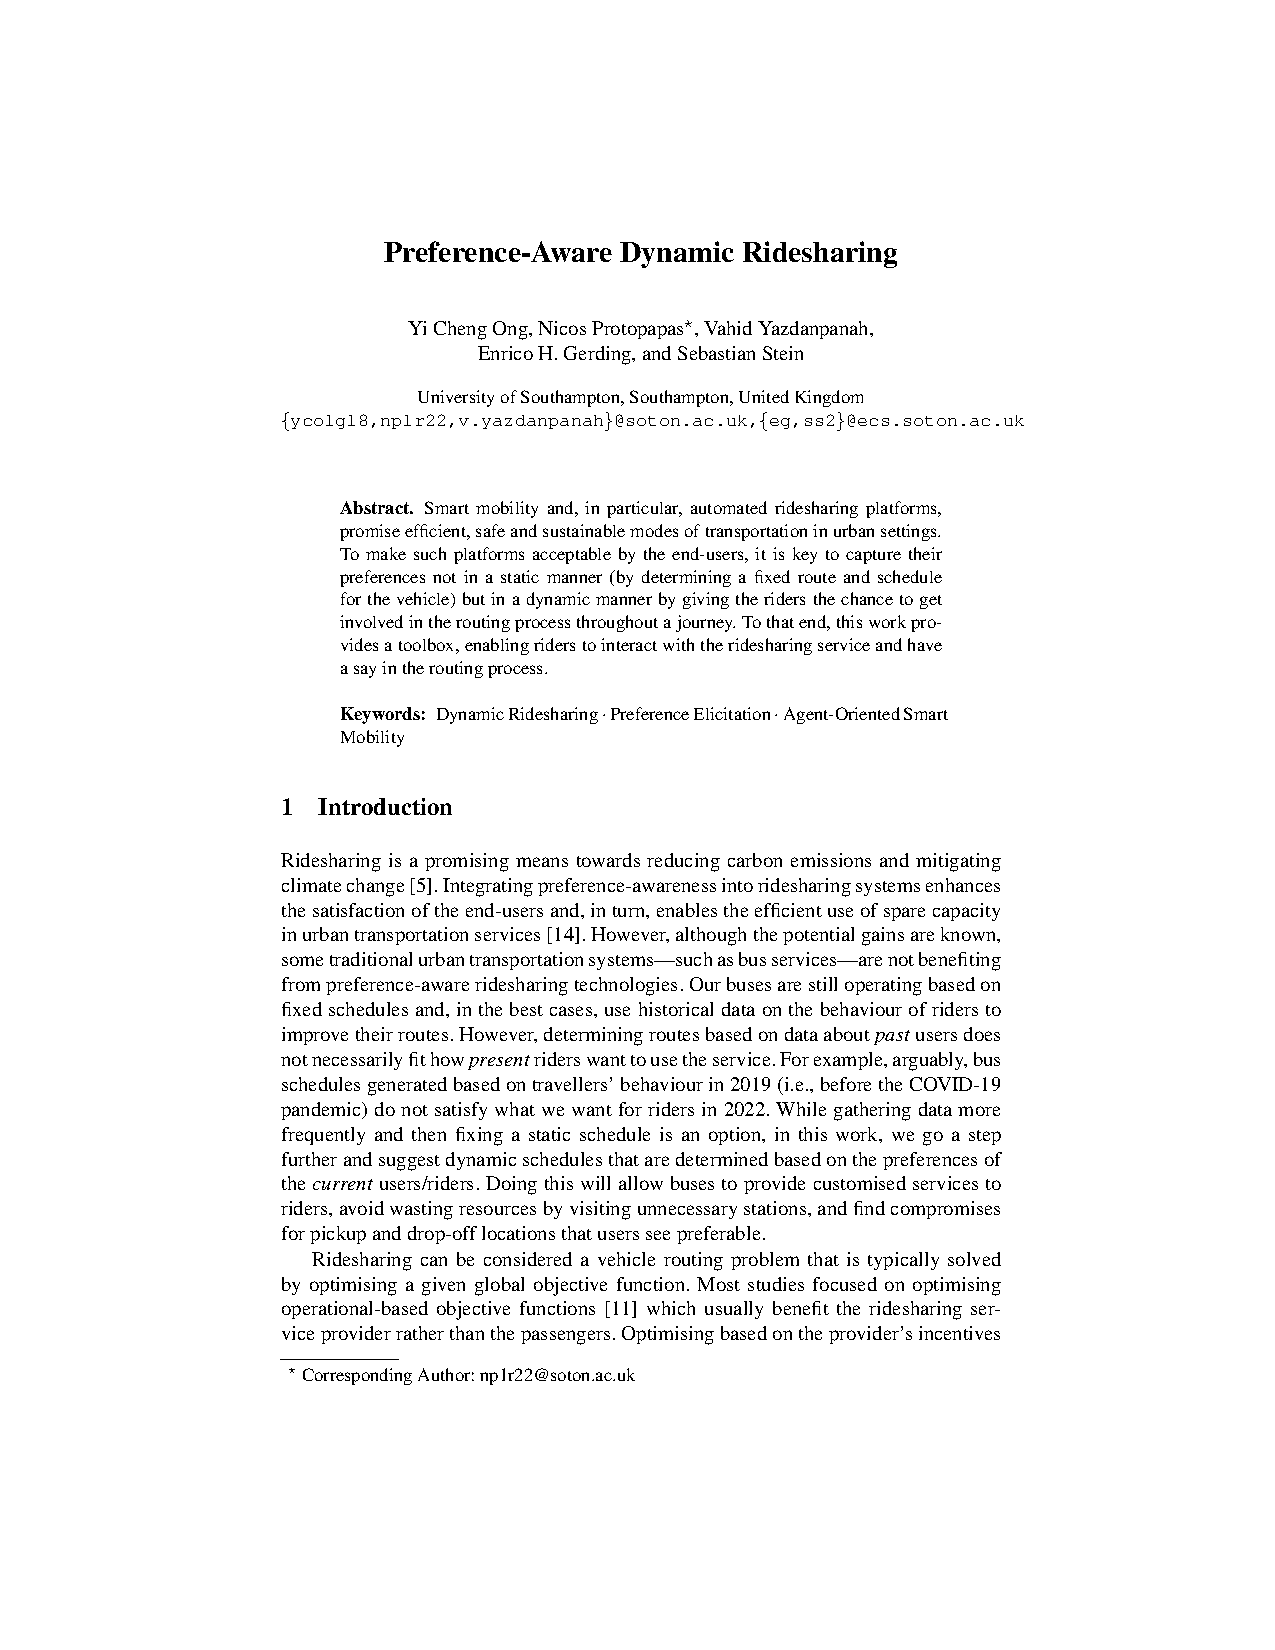
\includepdf[pages=-]{ABMUS2022_paper_6.pdf}
 
 \subsection{Multi-Agent Traffic Signal Control via Distributed RL with Spatial and Temporal Feature Extraction \\ Yifeng Zhang, Mehul Damani and Guillaume Sartoretti}
 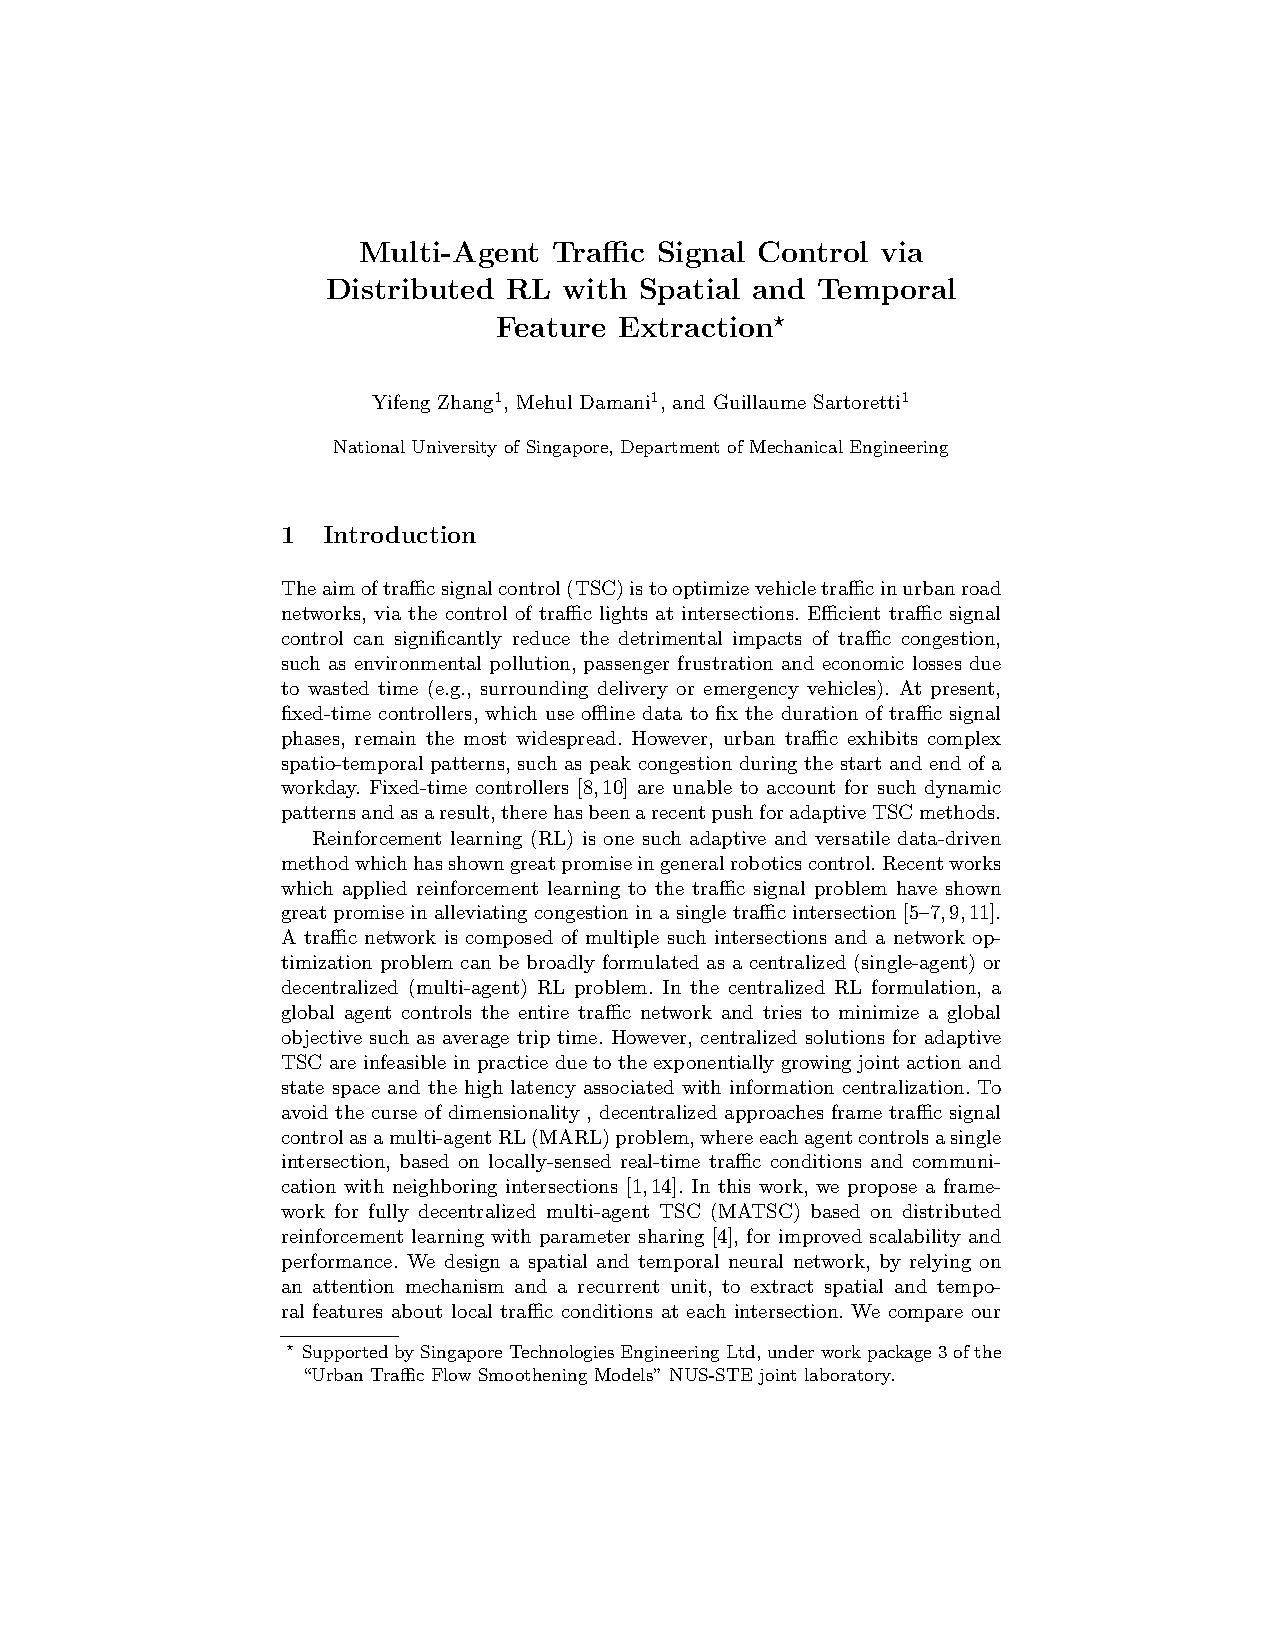
\includepdf[pages=-]{ABMUS2022_paper_7.pdf}
 

\end{document}
